\documentclass[]{article}
\usepackage[T1]{fontenc}
\usepackage{lmodern}
\usepackage{amssymb,amsmath}
\usepackage{ifxetex,ifluatex}
\usepackage{fixltx2e} % provides \textsubscript
% use upquote if available, for straight quotes in verbatim environments
\IfFileExists{upquote.sty}{\usepackage{upquote}}{}
\ifnum 0\ifxetex 1\fi\ifluatex 1\fi=0 % if pdftex
  \usepackage[utf8]{inputenc}
\else % if luatex or xelatex
  \ifxetex
    \usepackage{mathspec}
    \usepackage{xltxtra,xunicode}
  \else
    \usepackage{fontspec}
  \fi
  \defaultfontfeatures{Mapping=tex-text,Scale=MatchLowercase}
  \newcommand{\euro}{€}
\fi
% use microtype if available
\IfFileExists{microtype.sty}{\usepackage{microtype}}{}
\usepackage[margin=1in]{geometry}
\usepackage{longtable,booktabs}
\usepackage{graphicx}
% Redefine \includegraphics so that, unless explicit options are
% given, the image width will not exceed the width of the page.
% Images get their normal width if they fit onto the page, but
% are scaled down if they would overflow the margins.
\makeatletter
\def\ScaleIfNeeded{%
  \ifdim\Gin@nat@width>\linewidth
    \linewidth
  \else
    \Gin@nat@width
  \fi
}
\makeatother
\let\Oldincludegraphics\includegraphics
{%
 \catcode`\@=11\relax%
 \gdef\includegraphics{\@ifnextchar[{\Oldincludegraphics}{\Oldincludegraphics[width=\ScaleIfNeeded]}}%
}%
\ifxetex
  \usepackage[setpagesize=false, % page size defined by xetex
              unicode=false, % unicode breaks when used with xetex
              xetex]{hyperref}
\else
  \usepackage[unicode=true]{hyperref}
\fi
\hypersetup{breaklinks=true,
            bookmarks=true,
            pdfauthor={Brian C., James Q., Rohan F., Sharad G.},
            pdftitle={Sandwich Tycoon},
            colorlinks=true,
            citecolor=blue,
            urlcolor=blue,
            linkcolor=magenta,
            pdfborder={0 0 0}}
\urlstyle{same}  % don't use monospace font for urls
\setlength{\parindent}{0pt}
\setlength{\parskip}{6pt plus 2pt minus 1pt}
\setlength{\emergencystretch}{3em}  % prevent overfull lines
\setcounter{secnumdepth}{0}

\title{Sandwich Tycoon}
\author{Brian C., James Q., Rohan F., Sharad G.}
\date{}

\begin{document}

\begin{center}
\huge Sandwich Tycoon \\[0.2cm]
\end{center}
\begin{center}
\large \emph{Brian C., James Q., Rohan F., Sharad G.}\\[0.1cm]
\end{center}
\normalsize


\subsubsection{Preliminary Analysis}\label{preliminary-analysis}

After plotting histograms and scatterplots of the historical data, it
was evident that:

\begin{itemize}
\itemsep1pt\parskip0pt\parsep0pt
\item
  Demand can be modeled as a random variable.
\item
  Very often sandwich demand exceeded supply.
\item
  Daily sandwich demand was independent of previous demand.
\item
  Customer orders are independent of each other during the course of the
  day.
\item
  No obvious long-term demand trend upwards or downwards (linear
  regression, $a<.02$ and $r2<.0001$ for all types)
\end{itemize}

\subsubsection{Initial Graphs}\label{initial-graphs}

\includegraphics{./IS606_Sandwich_files/figure-latex/unnamed-chunk-21.pdf}
\includegraphics{./IS606_Sandwich_files/figure-latex/unnamed-chunk-22.pdf}
\includegraphics{./IS606_Sandwich_files/figure-latex/unnamed-chunk-23.pdf}

\subsubsection{Objective}\label{objective}

To maximize total sandwich profits over a 130-day period by estimating
probability of demand and producing a fixed or variable quantity of
supply.

\subsubsection{General Strategy}\label{general-strategy}

Sandwiches sold is a discrete variable and therefore can be estimated
using a probability mass function. We forecasted demand using two
different probability distributions. The first was to use the historical
frequency: This distribution would match the probability ($X=x$) of the
preceding period.

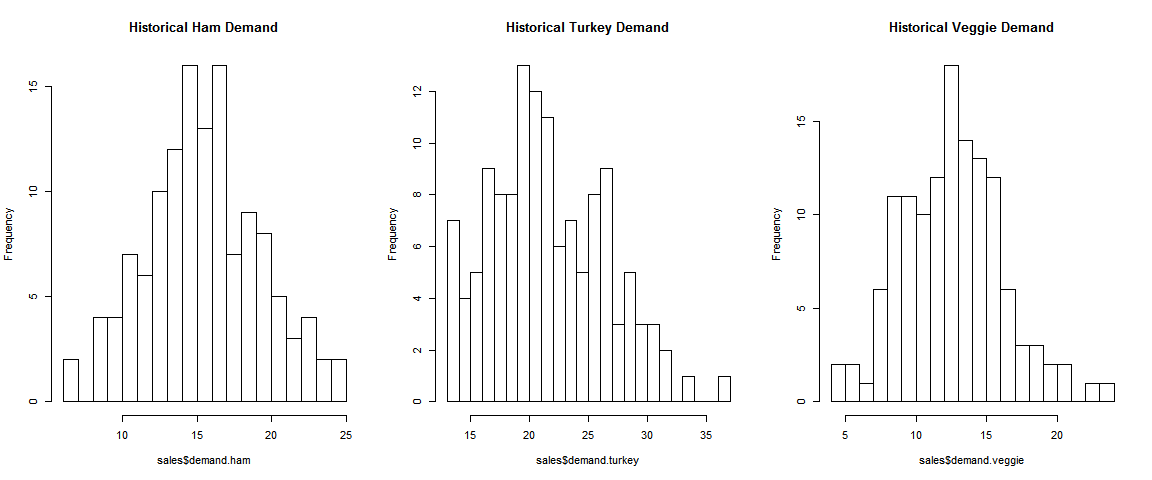
\includegraphics{./IS606_Sandwich_files/figure-latex/unnamed-chunk-3.pdf}

The second one is based on the frequency distribtutions suggest a
probability distribution. Since, there is no constraint on the number of
events and the outcomes are independent, we chose Poisson distribution
as a candidate. In order to use Poisson distribution, we calculated
lambda from historica data that gave us sandwich demand per day.

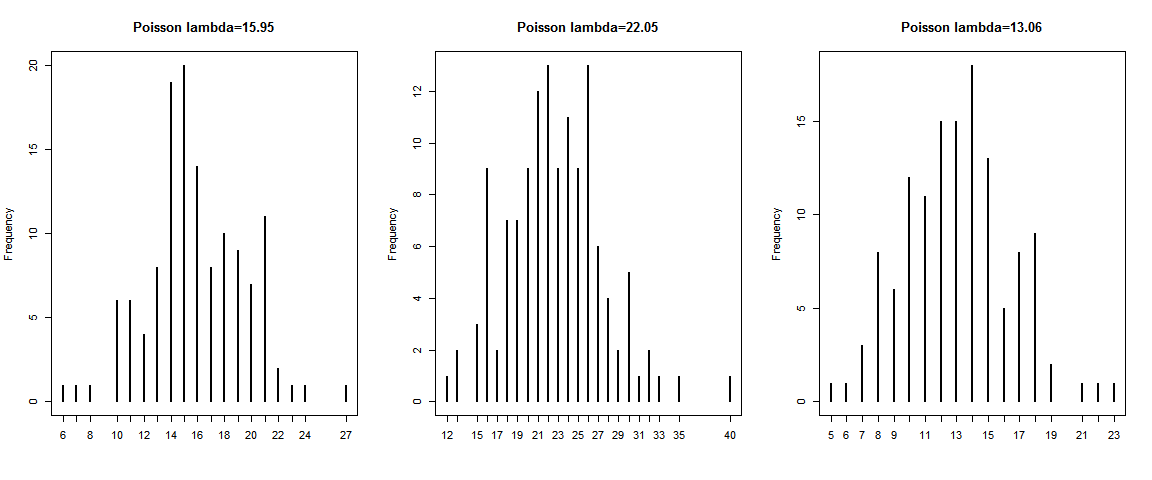
\includegraphics{./IS606_Sandwich_files/figure-latex/unnamed-chunk-4.pdf}

James previously supplied sandwiches at a mostly fixed amount. We used a
fixed supply model for the historical distribution but modeled the
poisson distribution under both fixed and variable supply assumptions.

A 130-day period was chosen to match the timeline of the given data.
This allows for direct benchmarking (given below assumptions) against 1)
profits that James actually made in the preceding 130 days, and 2) a
gold standard profit margin that was achievable over 130 days if supply
always met demand every day.

\subsubsection{General Assumptions}\label{general-assumptions}

\begin{itemize}
\itemsep1pt\parskip0pt\parsep0pt
\item
  Demand for each sandwich type is independent. What a customer orders
  is independent of what was ordered before.
\item
  Each customer only counts towards demand of one sandwich type.
  Therefore, if a customer wanted ham but it was sold out and turkey was
  bought instead, demand would count as 1 ham, 0 turkey. This means the
  sum of total demand equals the total number of customers who visited
  on a given day
\item
  Future demand will closely match historical demand. Again, there was
  no evident long-term trend and we have no information to assume a
  drastic drop or growth over the next 130 days (e.g.~more people in the
  building, other competition, vegan explosion, swine flu epidemic)
\item
  There are no added fixed costs to increasing supply (e.g.~hiring
  helpers, more preparation space/tools)
\item
  Supply goes to waste if not sold in a day. We vary this assumption in
  our second Poisson distribution model in that unsold sandwiches are
  reused (and thus increase future supply).
\end{itemize}

\subsubsection{Profit Results}\label{profit-results}

\paragraph{A) Previously achieved -
\$12,828}\label{a-previously-achieved---12828}

Given James' actual supply and demand over the 130-day period, he
achieved the following:

\begin{longtable}[c]{@{}llll@{}}
\toprule\addlinespace
Type & Revenue & Cost & Profit
\\\addlinespace
\midrule\endhead
Ham & \$12,012 & \$7,175 & \$4,837
\\\addlinespace
Turkey & \$14,066 & \$8,960 & \$5,106
\\\addlinespace
Veggie & \$5,960 & \$3,075 & \$2,885
\\\addlinespace
Total & \$32,038 & \$19,210 & \$12,828
\\\addlinespace
\bottomrule
\end{longtable}

\paragraph{B) Historical Probability Distribution -
\$13,858}\label{b-historical-probability-distribution---13858}

We used historical frequency of each demand amount to determine the
probability ($X=x$) of each sandwich sold on a given day. With this
probability distribution, we simulated 10,000 trials over a 130-day
period to get our demand estimate. Under our assumption of fixed supply,
we calculated the revenue, cost, and profit for each fixed number of
sandwiches produced (over the demand range of each sandwich type).

The results demonstrate that the optimal fixed number of sandwiches to
supply per day is equal to the expected value, which under a specific
frequency distribution is the highest frequency value (ham: $n=15$
$p=0.123$, turkey: $n=20$ $p=0.1$, veggie: $n=13$ $p=.138$).

\begin{longtable}[c]{@{}llll@{}}
\toprule\addlinespace
Type & Revenue & Cost & Profit
\\\addlinespace
\midrule\endhead
ham & \$11,765 & \$6,825 & \$4,940
\\\addlinespace
turkey & \$16,003 & \$10,400 & \$5,603
\\\addlinespace
veggie & \$7,540 & \$4,225 & \$3,315
\\\addlinespace
total & \$35,308 & \$21,450 & \$13,858
\\\addlinespace
\bottomrule
\end{longtable}

\paragraph{C) Poisson Distribution - Fixed Supply Without Storage
(unsold sandwiches are
wasted)}\label{c-poisson-distribution---fixed-supply-without-storage-unsold-sandwiches-are-wasted}

We assume that James will bring in a fixed amount every day and has no
way to store excess sandwiches. We choose 3 different models:

\begin{itemize}
\itemsep1pt\parskip0pt\parsep0pt
\item
  Using the lowest numbers from the data: 14 ham, 14 turkey, and 8
  veggie sandwiches
\item
  Using the higher numbers from the data: 18 ham, 20 turkey, and 10
  veggie sandwiches
\item
  Using the mean demand for each sandwich from the data: 16 ham, 22
  turkey, and 13 veggie sandwiches
\end{itemize}

Note: we do not show maximum demand model on this graph, since with no
storage, this reduces profits by a significantly wide margin.

\includegraphics{./IS606_Sandwich_files/figure-latex/unnamed-chunk-8.pdf}

\paragraph{D) Fixed Supply With Storage (unsold sandwiches are put back
into
supply)}\label{d-fixed-supply-with-storage-unsold-sandwiches-are-put-back-into-supply}

We assume that James will bring in a fixed amount every day but this
time does have a wat store excess sandwiches. We choose 4 different
models:

\begin{itemize}
\itemsep1pt\parskip0pt\parsep0pt
\item
  Using the lowest numbers from the data: 14 ham, 14 turkey, and 8
  veggie sandwiches
\item
  Using the higher numbers from the data: 18 ham, 20 turkey, and 10
  veggie sandwiches
\item
  Using the mean demand for each sandwich from the data: 16 ham, 22
  turkey, and 13 veggie sandwiches
\item
  Using the maximum demand model for each sandwich from the data: 25
  ham, 37 turkey, and 24 veggie sandwiches
\end{itemize}

\includegraphics{./IS606_Sandwich_files/figure-latex/unnamed-chunk-9.pdf}

\paragraph{E) Gold Standard - \$17,631}\label{e-gold-standard---17631}

This is the profit that would have been made if supply = demand each day
(variable supply model) so that no sandwich was wasted and every
customer was satisfied. Comparing the previous methods as percent of
gold standard achieved, we see the ``fixed supply at average demand, no
storage model'' yielded \textbf{78.2431\%} while the ``fixed supply at
average demand, storage model'' yielded \textbf{89.2119\%}.

\subsubsection{Recommendations}\label{recommendations}

\begin{itemize}
\itemsep1pt\parskip0pt\parsep0pt
\item
  If using a fixed supply with no storage, then it should be set to
  expected value of each demand variable (i.e., supply of ham, turkey
  and veggie sandwiches should be 16, 22, 13, respectively). This will
  show an immediate increase in profits.
\item
  Poisson distribution fit historical data very well - can use as
  distribution function going forward
\item
  Consider investing in fridge, etc. to prolong product shelf life.
  Without storage, when you over-shoot on supply (i.e.~customer demand
  is to the left of the mean), you lose money in waste. Having storage
  allows you to overshoot without having to bear that extra cost.
\item
  Being able to carry over supply day-to-day greatly increases expected
  profit
\item
  If overestimating demand, we recommend veggie because the profit
  margin is the same as turkey but the cost is the least.
\item
  If underestimate demand, we recommend turkey because the cost is the
  highest but the profit is same as veggie.
\end{itemize}

\subsubsection{Limitations}\label{limitations}

\begin{itemize}
\itemsep1pt\parskip0pt\parsep0pt
\item
  Simple model assuming external factors not changing
\item
  Will historical demand \textasciitilde{} Future demand?
\item
  Covariance. If no turkey is produced, could some/all switch to higher
  margin ham?
\item
  Fixed supply costs in real world would likely increase
\item
  In variable model, 3-day old sandwich is as `desirable' as fresh one
\end{itemize}

\end{document}
